\chapter{Decision-Theoretic Planning}
\label{ch:background}
% Introduction on what is Decision-Theoretic Planning
Automated \acrfull{acr:sdm} comprises the central problem of planning under uncertainty. 
\acrfull{acr:dtp} is concerned with the design of plans or \textit{policies} for settings in which uncertainty exists about the effects of actions, where the decision maker or \textit{agent} has incomplete information about the environment and its initial conditions, and where trade-offs need to be made between potentially conflicting objectives to determine an optimal course of action.
% <To be determined>
% Chapter organized as follows: section x....

\section{General Problem Formulation}
\label{sec:problem-formulation}
% Formulation of what kind of planning problems are considered in Decision-Theoretic Planning

The class of problems that are considered in \acrlong{acr:dtp} are those that require optimal stochastic control through the actions of decision maker(s), referred to as \textit{agent(s)}, in systems whose dynamics can be modeled as \textit{stochastic processes} \cite{Boutilier1999}.
The agent(s) in these systems sequentially need to choose from a set of actions that influence the system's behavior, consequently making the system switch from one state to another.
In these settings the system's current state and the agent's choice of action determines the probability distribution over the states the system might reach next.
In addition, the agent(s) might be uncertain about the system's current state, implying the need to infer from observations and making decisions based on probabilistic estimates of the system's state.

Typically the problems under consideration involve certain objectives to be achieved (e.g., tasks to be fulfilled) or properties to be satisfied (e.g., avoiding certain system states). 
Therefore the agent should decide on a optimal plan or \textit{policy} which makes it most likely for the system to reach its targets, while minimizing the risk of producing undesirable states and the accompanied costs of the policy.
To find such a policy for \acrlong{acr:sdm} problems, a typical approach is to first setup a probabilistic model of the system and then apply a \acrshort{acr:dtp} algorithm on this model.
This probabilistic model comprises a system representation which defines the state space in terms of a set of multi-valued features, the set of actions for the agent to select together with the associated uncertainty defined by transition-probabilities, and a goal specification or performance metric regularly expressed by means of a reward structure.

Overall \acrshort{acr:dtp} aims to devise planning algorithms for planning under uncertainty, a problem that is addressed in numerous different fields of research such as AI planning and control theory.
In particular difficulties arise when planning techniques are applied to determine courses of action for real-world settings, such as % TODO

\section{System Representations: Markov Models}
\label{sec:system-representation}
% Definitions of Markov Models relevant as probabilistic models for planning under uncertainty

As the class of problems considered in \acrshort{acr:dtp} oft to present considerable structure, there exist various proposed solutions for planning under uncertainty that apply model-based approaches.
This type of decision-theoretic planner uses a stochastic model of the environment in which the agent operates, which compasses the uncertainty that is associated with the agent's actions, observations and the exogenous events that might occur.
Typically the uncertainty is modeled by establishing a \textit{state space} for the system accompanied by a set of possible \textit{transitions} between the states that might be induced with a certain probability by an agent executing \textit{actions}.
The most common types of stochastic models that are used in \acrshort{acr:dtp} are called \textit{Markov Models} (sometimes also referred to as \textit{Markovian Models}), which has been motivated by their success in other fields such as speech recognition \cite{baker1992large, gales2008application, rabiner1989tutorial} and reinforcement learning techniques \cite{Brafman2002}. %TODO Add more citations for RL
A Markov Model is a stochastic model in which the future states only depend on a limited number of prior observations. In fact, mostly processes or systems are modeled by Markov Models that satisfy the \textit{Markov Property}, which means that the state transitions are independent of any previous states or agent actions.

In the remainder of this section the most common types of discrete-state Markov Models are discussed one by one, starting from the fundamental models known as \textit{Markov Chains} in \autoref{subsec:markov-chains}, followed by their extension of \textit{\acrfullpl{acr:hmm}} in \autoref{subsec:hidden-markov-models}.
This again is followed by a discussion of the discrete-state Markov Models most relevant in \acrshort{acr:dtp}, being \textit{\acrfullpl{acr:mdp}} in \autoref{subsec:mdps} and their extension of \textit{\acrfullpl{acr:pomdp}} in \autoref{subsec:pomdps}.

\subsection{Markov Chains}
\label{subsec:markov-chains}
% Markov Chains: States and Transitions

% See summary barberBRML2012

\begin{figure}[ht!]
	\captionsetup[subfigure]{justification=centering}
	\centering
	\subcaptionbox{First-order Markov Chain.\label{fig:markov-chains-first-order}}{\begin{tikzpicture}[->,>=stealth',auto,node distance=2cm]
		\tikzstyle{every state}=[fill=white,draw=black,text=black,scale=1,double]	% thick
		\node[state] (s1) {$s_1$};
		\node[state] (s2) [right of=s1] {$s_2$};
		\node[state] (s3) [right of=s2] {$s_3$};
		\coordinate (con) at (0,2);
		\path
		(s1)
		edge node {} (s2)
		(s2)
		edge node {} (s3)
		(s3);
		\draw [->, dashed, shorten >=0pt] (s3) to[right] node[auto] {} ++(1.3,0)
		;
		\end{tikzpicture}} \quad
		\subcaptionbox{Second-order Markov Chain.\label{fig:markov-chains-second-order}}{\begin{tikzpicture}[->,>=stealth',auto,node distance=2cm]
		\tikzstyle{every state}=[fill=white,draw=black,text=black,scale=1,double]	% thick
		\node[state] (s1) {$s_1$};
		\node[state] (s2) [right of=s1] {$s_2$};
		\node[state] (s3) [right of=s2] {$s_3$};
		\node[state] (s4) [right of=s3] {$s_4$};
		\path
		(s1)
		edge node {} (s2)
		(s2)
		edge node {} (s3)
		(s1)
		edge [bend left] node {} (s3)
		(s3)
		edge node {} (s4)
		(s2)
		edge [bend left] node {} (s4)
		;
		\draw [->, dashed, shorten >=0pt] (s4) to[right] node[auto] {} ++(1.3,0)
		;
		\end{tikzpicture}}
	\caption{Graphical representation of different types of Markov Chains.}
	\label{fig:markov-chains}
\end{figure}

\subsection{Hidden Markov Models}
\label{subsec:hidden-markov-models}
% Hidden Markov Models: Observations (partially observable) 
% also called latent
% inference problems
% shortly discuss the succesful applications see \cite{barberBRML2012} speech recognition, object tracking, genetic sequence analysis and add citations to the corresponding works

%

\subsection{Markov Decision Processes}
\label{subsec:mdps}

% MDPs: Actions --> Is a probabilistic model			% Driven by the actions of an agent
% 	(Exogeneous) events
% Policies

%

\subsection{Partially Observable MDPs}
\label{subsec:pomdps}

% Observations: .. POMDP
% Reward Models and Value Functions

% 

\subsection{Other Markov Models and Related State-Space Models}
\label{subsec:other-markov-models}
Apart from the discrete-state Markov Models that were discussed in this section, there exist numerous other types of Markov Models and closely related State-Space Models (SMMs), including among others the following:%, including continuous-state Markov Models (e.g., Linear Dynamical Systems with a Gaussian state-space \cite{Minka1999,barberBRML2012}) and other specialized variations. 

\begin{description}
	\item[Factored Markov Decision Process (FMDP)] An extension of the MDP-model that allows for compact representation of states, transitions and rewards \cite{Degris2010}.
	\item[To be determined] To be determined 
	\item[Linear Dynamical System (LDS)] A continuous-state State-Space Model with linear dynamics, Gaussian state-space and the assumption of hidden variables as in \acrshortpl{acr:hmm} \cite{Minka1999, barberBRML2012, Ghahramani2000}.
\end{description}

As the remaining chapters only consider systems and processes that are modeled using discrete-state Markov Models, these variations will not be further discussed in more detail.

\section{Learning Optimal Policies}
\label{sec:planning}

% Sutton and Barto (1998/2012) describe two approaches for rl solutions when the transition and reward functions are not known	(Learning the Structure of Factored Markov Decision Processes inReinforcement Learning Problems)
% See chapter 8.2, show an adapted version of the figure and explain advantages and disadvantages

\subsection{Model-Free Planning Techniques}		% Also referred to as Direct or value-based approaches
\label{subsec:model-free-planning}

% 

\subsection{Model-Based Planning Techniques}	% Also referred to as Indirect approaches
\label{subsec:model-based-planning}

\begin{figure}[ht!]
	\centering
	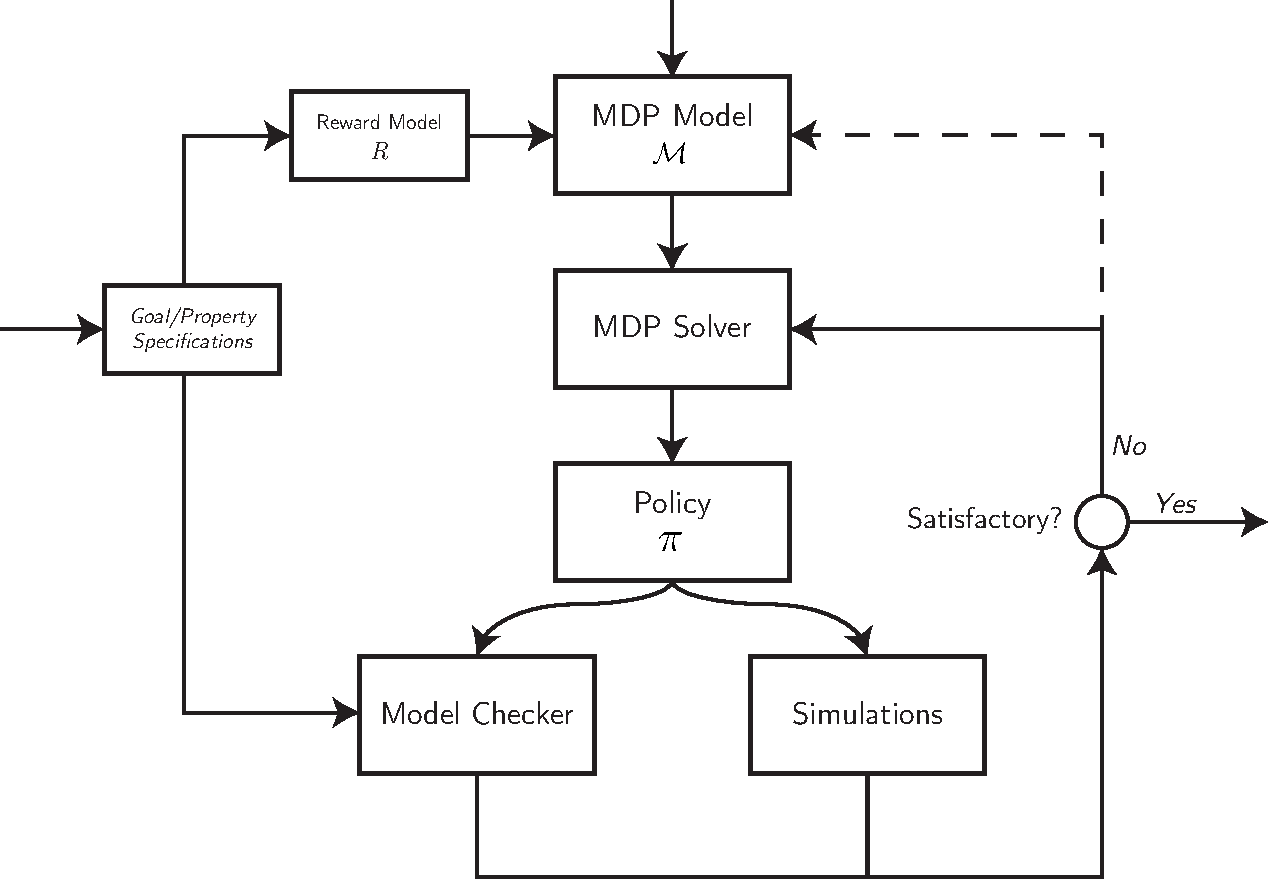
\includegraphics[width=\textwidth]{mdp-planning-diagram}
	\caption{Block diagram of the generic routine employed in model-based MDP planning techniques.}
	\label{fig:model-based-routine}
\end{figure}
% Planning algorithms for MDPs
% Planning algorithms for POMDPs

% \subsection{Integrated Architectures}
% Dyna Architecture -- combines model-learning and direct/value-based approaches, applies these iteratively even in execution of the agent --> 'hybrid' approach?
	% See "Integrated Learning and Planning" Lecture sheets by David Silver	[Integrated Architecture]
	% 

% 7.9.2








% perceptual aliasing!!!!!!